\chapter{PROBLEM}

The basic problem in this thesis is how to find appropriate job descriptions by user's r\'esum\'e. If we take the r\'esum\'e as a query and the job descriptions as documents, we need to build an information retrieval model to get the most relevance documents.  The JobFinder will parse the job descriptions to the job models, and store them in the database. When a user searches the jobs by their r\'esum\'e in the system, the system will compare the similarity values between the r\'esum\'e and the job models, and return the jobs sorted by their similarity values.

The core idea of our algorithm is calculate similarity between the r\'esum\'e model and job model.
We give a formal definition of our problem. All of the notations will be used frequently throughout the thesis.

We use $r$ to denote the user's r\'esum\'e model, which has some features $r_i$ like their academic degree, their major, their skills and so on. The symbol $J$ is the set of job models stored in the database, and $j$ is a job model in the set $J$. The similarity function $sim(r, j)$ gives the similarity values between r\'esum\'e $r$ and job $j$. The return list of search function $search(r,J)$ will calculate all the similarity value in the database, and the result of the function will be the job description list ranked by their similarity values. The equation of how to calculate similarity value is given below:

$$ sim(r, j) = \sum_{i=1}^{n} simfun_i(r_i,j_i) \times w_i $$

The value of $sim(r, j)$ is the summation of the similarity values of different fields times their corresponding weights. Different fields like major and skills,  may have different functions to calculate their similarity values. We will describe the similarity functions of individual fields in later parts.


\chapter{System Overview}

\section{System Overview}
The system uses information extraction technique to parse job descriptions and r\'esum\'es, and it gets information such as skills, job titles and education background. The information is used to create the models of job openings and job seekers. A domain specific ontology is used to construct the knowledge base, which includes the taxonomies that support r\'esum\'e-job matching.

The models of r\'esum\'e includes job seekers' specialties, working experience and education background, and all the fields are extracted from their r\'esum\'es. The job models are extracted from job descriptions, and they have the same information fields as the r\'esum\'e models.  When a job seeker searches the jobs by their r\'esum\'e, the system calculates the similarity between the r\'esum\'e model and job models, then gives every job model a similarity value.

\section{System Architecture}

Figure~\ref{fig:Pipeline} shows the architecture of the whole system, which includes such modules:

\begin{enumerate}
    \item The Web Crawler can access and download all new IT job opening web pages from indeed.com everyday.
    \item The Job Parser can parse the job opening web pages, extract the information and create the job models.
    \item The Resume Parser is much like the Job Parser; it parses the r\'esum\'es and creates the r\'esum\'e models.
    \item All the job descriptions and job models are stored in the database.
    \item When a user searches  the jobs with their r\'esum\'e, the Ontology Matcher calculates the similarity values of jobs in the database and returns the jobs ranked by their similarity values.
\end{enumerate}

\begin{figure}[htbp]
  \centering
  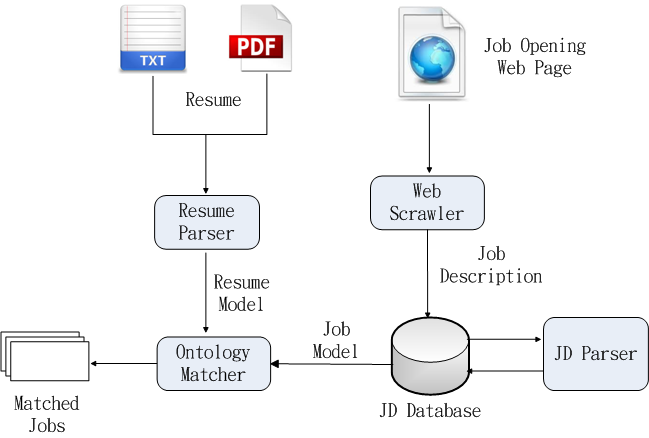
\includegraphics[scale=0.5]{images/arch.png}
  \caption{System Architecture}
  \label{fig:arch}
\end{figure}

\section{System Implementation}

We will describe some implementation details here. The whole system is implemented in Python and uses some third party libraries and frameworks. We used Flask, a lightweight web framework, to build the web application. We used Rdflib as the Web Ontology Language (OWL) file parser, Python Lex-Yacc (PLY) as the token regular expression compiler, whoosh as the inverted index builder and Beautiful Soup as the HTML parser.  All the jobs got by the Web Crawler are stored in the MongoDB NoSQL database.  For the natural language processing procedure, we used Natural Language Toolkit (NLTK), a  natural language processing library, to extract and  tokenize the sentences.

\section{System Interface}

The system provides some interfaces to end users. The most important interfaces are the web pages like: reviewing all the jobs in the database, searching the jobs by keyword (Figure~\ref{fig:joblist}),  uploading users' r\'esum\'es (Figure~\ref{fig:upload_resume}),  matching the jobs with a r\'esum\'e (Figure~\ref{fig:match_resume}) and searching the jobs with both keyword and the r\'esum\'e (Figure~\ref{fig:keyword_resume}).

\begin{figure}[htbp]
  \centering
  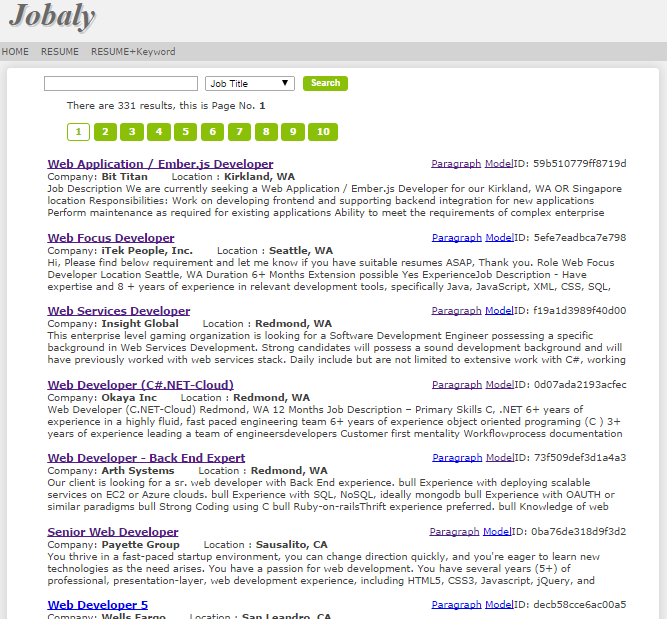
\includegraphics[scale=0.5]{images/joblist.png}
  \caption{Job Description List}
  \label{fig:joblist}
\end{figure}


\begin{figure}[htbp]
  \centering
  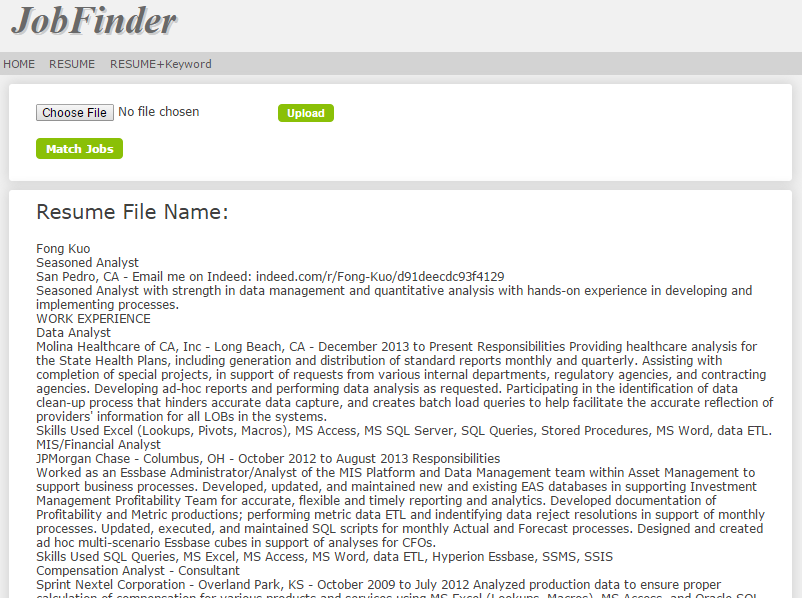
\includegraphics[scale=0.5]{images/upload_resume.png}
  \caption{Upload Resume}
  \label{fig:upload_resume}
\end{figure}

\begin{figure}[htbp]
  \centering
  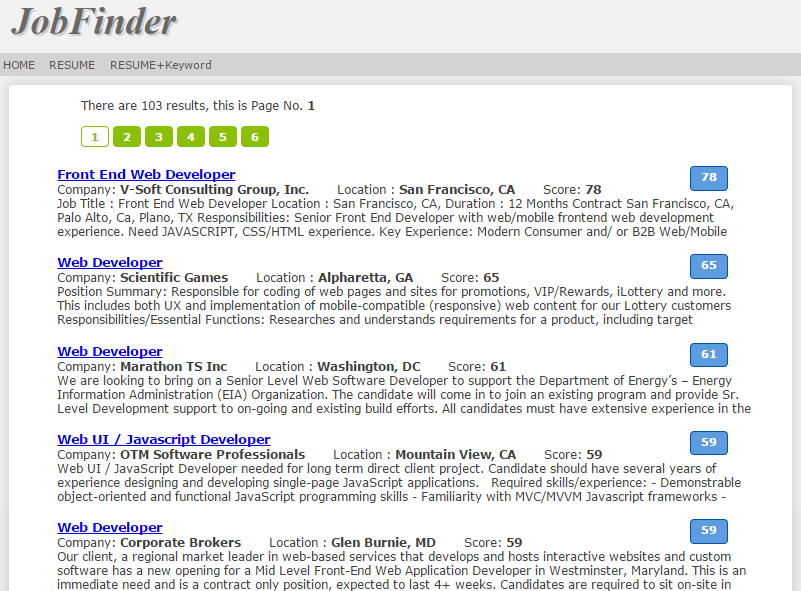
\includegraphics[scale=0.5]{images/match_resume.png}
  \caption{Resume Job matching }
  \label{fig:match_resume}
\end{figure}

\begin{figure}[htbp]
  \centering
  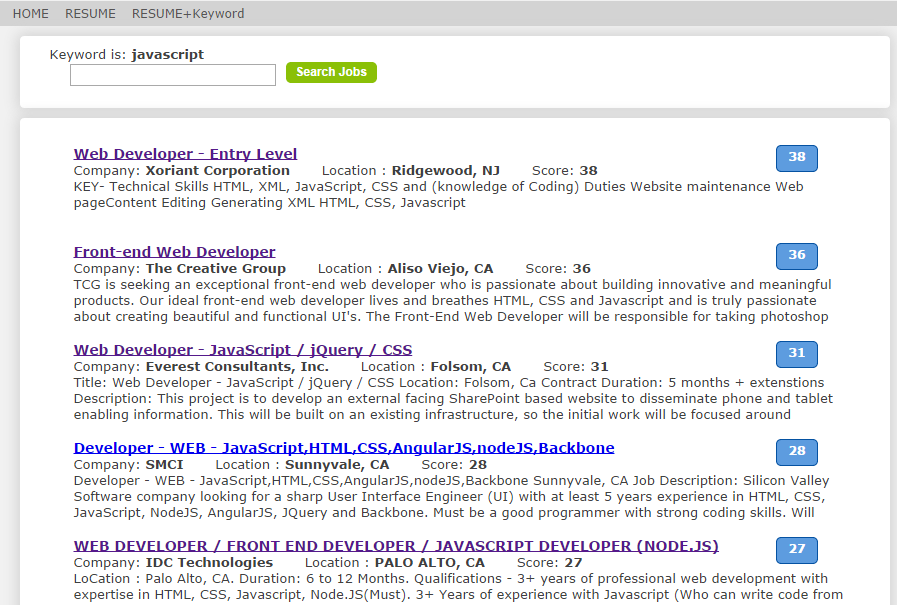
\includegraphics[scale=0.5]{images/keyword_resume.png}
  \caption{Combine the Keyword and Resume Matching}
  \label{fig:keyword_resume}
\end{figure}






